% Section 7.2: case (i), equal inversion cost. Facts: log items 59-62 (Q2 pairs), 104, 110-112; figures F8, F10a/b; results of run A and offline moves 24 Nov.
\subsection{Case (i): moving the sensors}\label{sec:case-i}
\begin{notes}
\item Pre-registered: gradient vs random moves, 13 pairs: gradient ranks higher in 10 of 13 (4 shots 3/3, 2 shots 4/5, 1 shot 3/5); 7 of 10 on the pairs specified in advance ($p=0.17$). With 4 shots only gradient moves find D4.
\item Against static 30 points (exploratory): mean found 5.00 / 4.40 / 4.20 vs 3.88 / 3.43 / 3.43 at 1\,\% rate (MWU $p=0.001$, paired 11/2/0); with the fixed-amplitude rule 5.00 / 4.20 / 3.40 ($p=0.021$, paired 8/4/1); random moves gain little ($p=0.18$ / 0.22): the gain comes from the direction, not the extra measurements.
\item Disclose: random moves have matched path lengths but smaller net displacement (13--14 vs 24--29\,mm).
\item Reference dense static scans (4 shots): regular 110 points 5/5, 26 false indications; the gradient array matches detection but not false indications (64--240).
\item \note{24 Nov}: all visited positions ($\approx$145) inverted at once vs static of the same size (mj, rg143); offline moves (designed on the background) vs gradient moves = value of adaptivity.
\item Figures: F10a row (i), F10b panel (i); sensor paths in Sec.~\ref{sec:paths}.
\item \textbf{24 Nov results}: moves planned beforehand (offline, best-case background model calibrated on the full defect scan) match gradient moves: same start 2/10/1 under every rule; 1\,\%: offline 4.67 / 4.40 / 4.20 vs gradient 5.00 / 4.40 / 4.20. Both beat random (offline vs random 7/5/1, $p=0.035$) and static 30 (11/2/0). Wording: the adaptive design matches a best-case design planned beforehand, without needing a prior model or design campaign.
\item Sweep geometry: designed moves keep their direction (cos 0.71--0.99) and end 23--35\,mm from their start; random moves wander (cos 0) and end 12--15\,mm away, at equal path length. A property of the design; direction vs distance not separated (disclose; no fixed-heading test).
\item Case (iv), $\approx$145 points, one-pass inversion on both sides: gradient-visited vs jittered static of the same size, v3 mean found 5.00 / 4.60 vs 4.33 / 4.80 (4 / 2 shots), all five at 4 shots 3/3 vs 1/3; false indications 66 / 137 vs 32 / 54; regular 143-point grid 5/5, 90 / 116. Competitive with uniform coverage, better on D4 at 4 shots, noisier background. At 1\,\% everything is at the ceiling.
\item F10a rows: (i) gradient, planned beforehand (blue), random (grey); (iv) gradient-visited and random-visited vs same-size static.
\end{notes}
\begin{figure}[ht]\centering
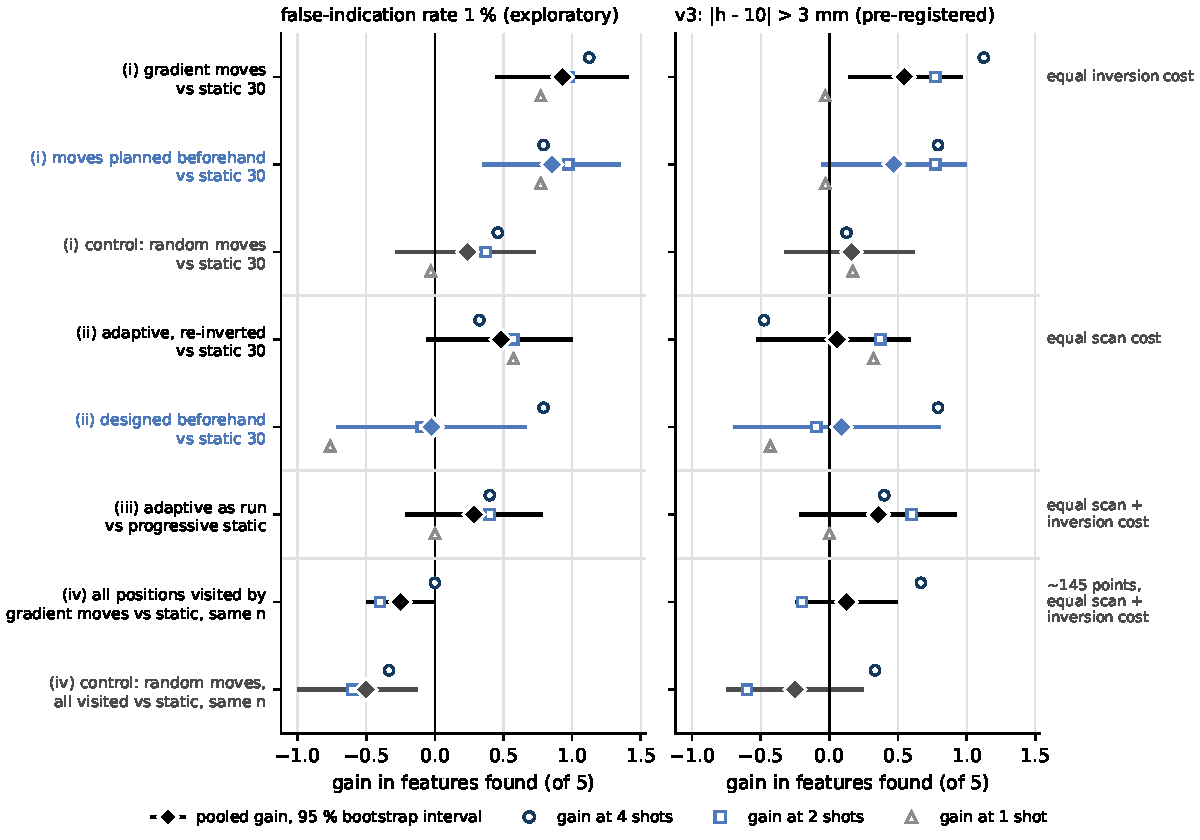
\includegraphics[width=0.8\linewidth]{F10a_funnel.pdf}
\caption{\textbf{Where the design helps: from relaxed to strict} (exploratory). Gain in features found (of 5) of the designed variant over its baseline; diamonds: pooled gain with 95\,\% bootstrap interval; open markers: gain at 4, 2 and 1 shots. Left: fixed 1\,\% false-indication rate; right: v3 (pre-registered). (i) equal inversion cost: 30 sensors moved along the illumination gradient vs static 30 points; blue: the same moves planned beforehand on a best-case model (calibrated on the full defect scan); grey: random moves. (ii) equal scan cost: adaptive points re-inverted in one pass; blue: 30 points designed beforehand. (iii) equal scan and inversion cost. (iv) about 145 points: all positions visited by the moving arrays, inverted in one pass, vs a static layout of the same size (4 and 2 shots).}\label{fig:funnel}
\end{figure}

\begin{figure}[ht]\centering
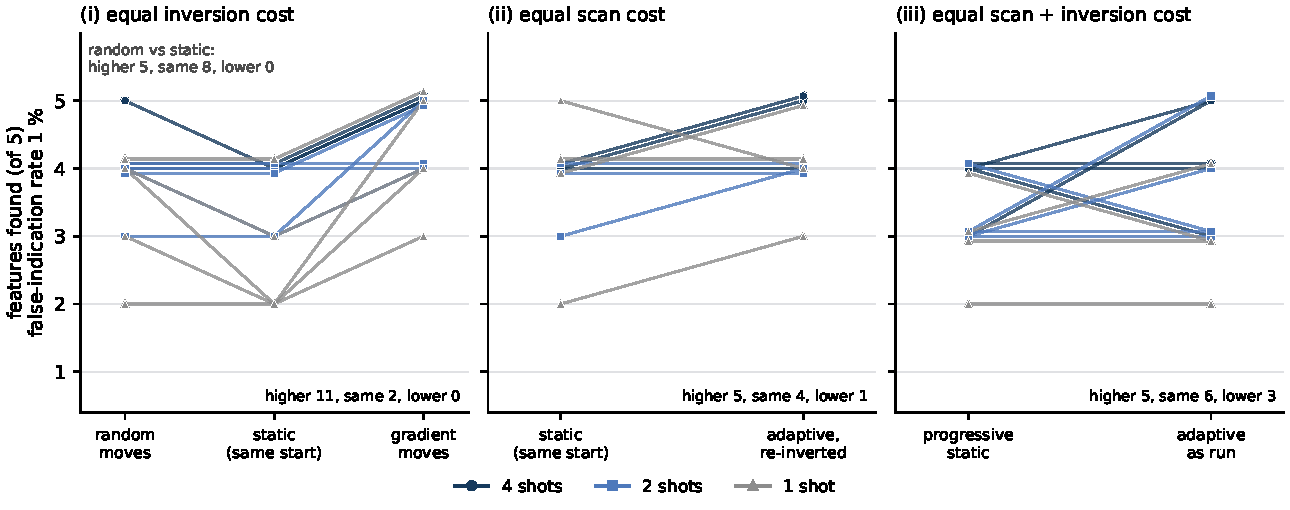
\includegraphics[width=\linewidth]{F10b_slopes.pdf}
\caption{\textbf{Paired view of Fig.~\ref{fig:funnel}} (1\,\% false-indication rate). Each line is one start layout, from its baseline to its designed variant; counts of start layouts that find more, the same or fewer features.}\label{fig:slopes}
\end{figure}

